\documentclass[11pt,a4paper]{scrarticle}
\usepackage[utf8]{inputenc}
\usepackage{cmap}
\usepackage[T2A]{fontenc}
\usepackage[russian]{babel}
\usepackage{amsmath,amssymb,amsthm,mathtools}
\usepackage{array}

\usepackage{indentfirst}
\usepackage{xcolor,graphicx, tikz, wrapfig}
\usepackage{longtable}
\usepackage{placeins}

\usepackage{minted}
\usemintedstyle{vs}

\usepackage[left=2cm,right=2cm,top=2cm,bottom=2cm,bindingoffset=0cm]{geometry}

\usepackage[unicode]{hyperref}
\definecolor{linkcolor}{HTML}{0000E6}
\definecolor{urlcolor}{HTML}{0000E6}
\definecolor{citecolor}{HTML}{0000E6}
\hypersetup{pdfpagemode=None,linktoc=page,citecolor=citecolor,linkcolor=linkcolor,urlcolor=urlcolor,colorlinks=true}

\theoremstyle{definition}
\newtheorem{subtask}{Пункт}

\DeclareMathOperator*{\argmax}{arg\,max}
\DeclareMathOperator*{\argmin}{arg\,min}
\newcommand{\floor}[1]{\left\lfloor #1 \right\rfloor}
\newcommand{\ceil}[1]{\left\lceil #1 \right\rceil}


\setlength{\parindent}{1cm}

\author{Клычков Максим Дмитриевич}

\begin{document}

\centerline{\textbf{\huge Алгоритмы и структуры данных-1}}
\centerline{\textbf{SET 3. Задача A3.}}
\begin{flushright}
	\emph{Осень 2024. Клычков М. Д.}
\end{flushright}

\begin{itemize}
	\item ID посылки по задаче \texttt{A1i}: \href{https://dsahse.contest.codeforces.com/group/NOflOR1Qt0/contest/565612/submission/292810314}{292810314}
	\item \href{https://github.com/maklybae/algorithms/tree/main/set03/a3}{Ссылка на репозиторий \texttt{GitHub}}
\end{itemize}

\subsection*{Внутренняя инфраструктура для экспериментального анализа}

Внутренняя инфраструктура для экспериментального анализа практически полностью была скопирована из предыдущей задачи. Из изменений добавился только общий генератор случайных чисел, распространяющийся на весь проект (это позволительно, так как мы запускаем программу в одном потоке).

Были реализованы классы \texttt{ArrayGenerator} и \texttt{SortTester} для организации удобного замера работы алгоритмов.

\begin{figure}[htp]
	\centering
	\inputminted[linenos,fontsize=\small]{cpp}{../analyze/generator.h}
	\caption{\texttt{ArrayGenerator Header File}}
	\label{code:generator-h}
\end{figure}
\FloatBarrier

\begin{figure}[htp]
	\centering
	\inputminted[linenos,fontsize=\small]{cpp}{../analyze/generator.cpp}
	\caption{\texttt{ArrayGenerator Cpp File}}
	\label{code:generator-cpp}
\end{figure}
\FloatBarrier

\begin{figure}[htp]
	\centering
	\inputminted[linenos,fontsize=\small]{cpp}{../analyze/tester.h}
	\caption{\texttt{SortTester Header File}}
	\label{code:tester-h}
\end{figure}
\FloatBarrier

\begin{figure}[htp]
	\centering
	\inputminted[linenos,fontsize=\small]{cpp}{../analyze/tester.cpp}
	\caption{\texttt{SortTester Cpp File}}
	\label{code:tester-cpp}
\end{figure}
\FloatBarrier

\begin{figure}[htp]
	\centering
	\inputminted[linenos,fontsize=\small]{cpp}{../analyze/random_utils.h}
	\caption{\texttt{Random Utils Header File}}
	\label{code:random-h}
\end{figure}
\FloatBarrier

В функции \texttt{main()} происходит создание сразу трех объектов \texttt{SortTester}. Каждый запуск происходит по три раза на каждом из тестеров, затем результаты усредняются.

\emph{Некоторые замечания}: эта реализация не является оптимальной по крайней мере потому, что один и тот же код вызова сортировок повторятся для каждого алгоритма, однако было принято решение оставить такую реализацию, так как она уж точно не содержит никаких подводных камней, которые могут повлиять на временную оценку.

\subsection*{Анализ}

Для построения графиков использовался язык \texttt{Python}.

Сначала проанализируем каждый алгоритм сортировки по отдельности. Начнем с \texttt{QuickSort}.

\begin{figure}[htp]
	\centering
	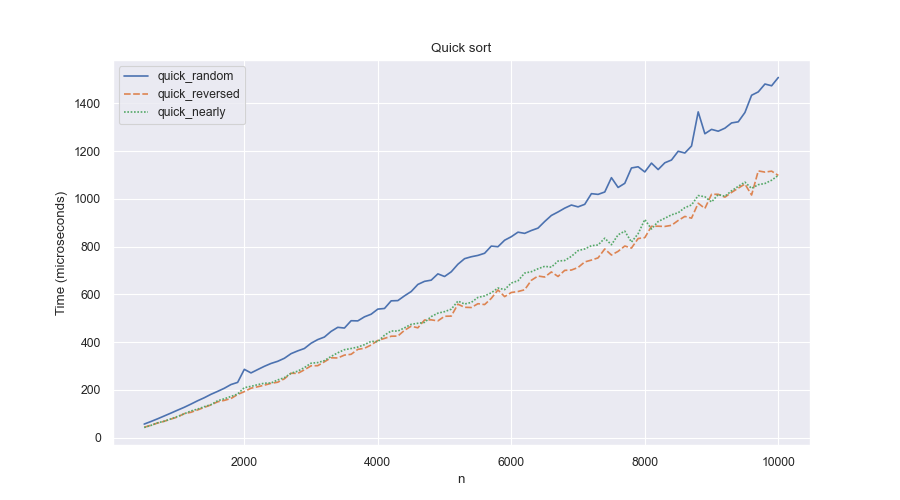
\includegraphics[width=\textwidth]{../static/quick.png}
	\caption{\texttt{QuickSort}}
	\label{fig:quick}
\end{figure}
\FloatBarrier

Можем заметить, что сортировка случайно заполненного неупорядоченного массива $\approx 1.33$~раза больше, чем сортировка почти упорядоченного по неубыванию и упорядоченного по невозрастанию массивов, время сортировки которых при равном $n$ приблизительно равны.

Казалось бы, сортировка почти упорядоченного массива должна лидировать по времени исполнения, однако при случайно выбранном элементе \texttt{pivot} это не так. Действительно, при выборе крайних элементов в качестве \texttt{pivot} приходится совершать большое количество перестановок элементов, которые сильно влияют на производительность. Во избежании такого поведения иногда применяют алгоритм \texttt{MedianOfThree} для выбора не случайного значения \texttt{pivot}, а заданного по определенному правилу.

Рассмотрим \texttt{IntroSort}.

\begin{figure}[htp]
	\centering
	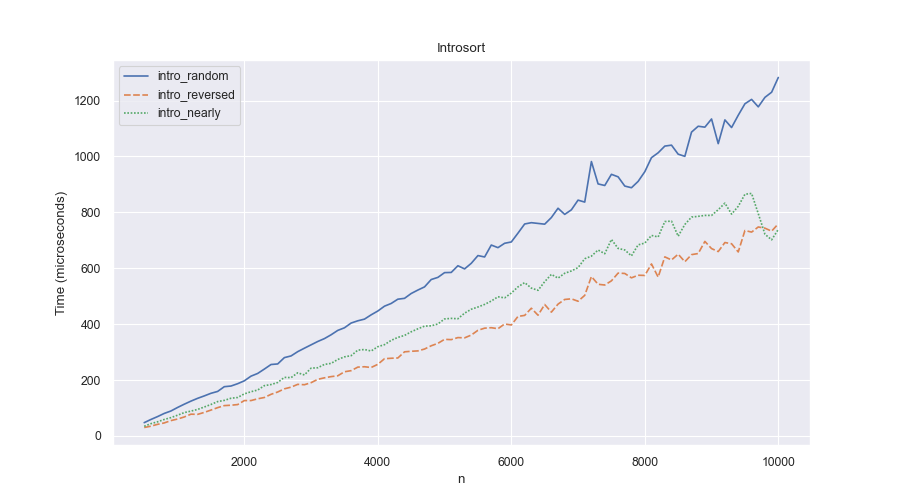
\includegraphics[width=\textwidth]{../static/intro.png}
	\caption{\texttt{IntroSort}}
	\label{fig:quick}
\end{figure}
\FloatBarrier

На этом графике наблюдается та же ситуация --- случайно заполненный массив «проигрывает» по времени двум другим видам массивов. Также здесь наблюдается более сильное расхождение по времени между обратно отсортированными и почти отсортированными массивами.

Лучший результат отсортированных по невозрастанию массивов может быть обеспечен тем, что при переходе на \texttt{HeapSort} \texttt{BuildMaxHeap} отрабатывает быстрее на такого рода массивах, но только в пределах скрытых констант, на асимптотику это никак не влияет.\pagebreak

Теперь же перейдем к сравнению двух алгоритмов: \texttt{IntroSort} и \texttt{QuickSort}.

\begin{figure}[htp]
	\centering
	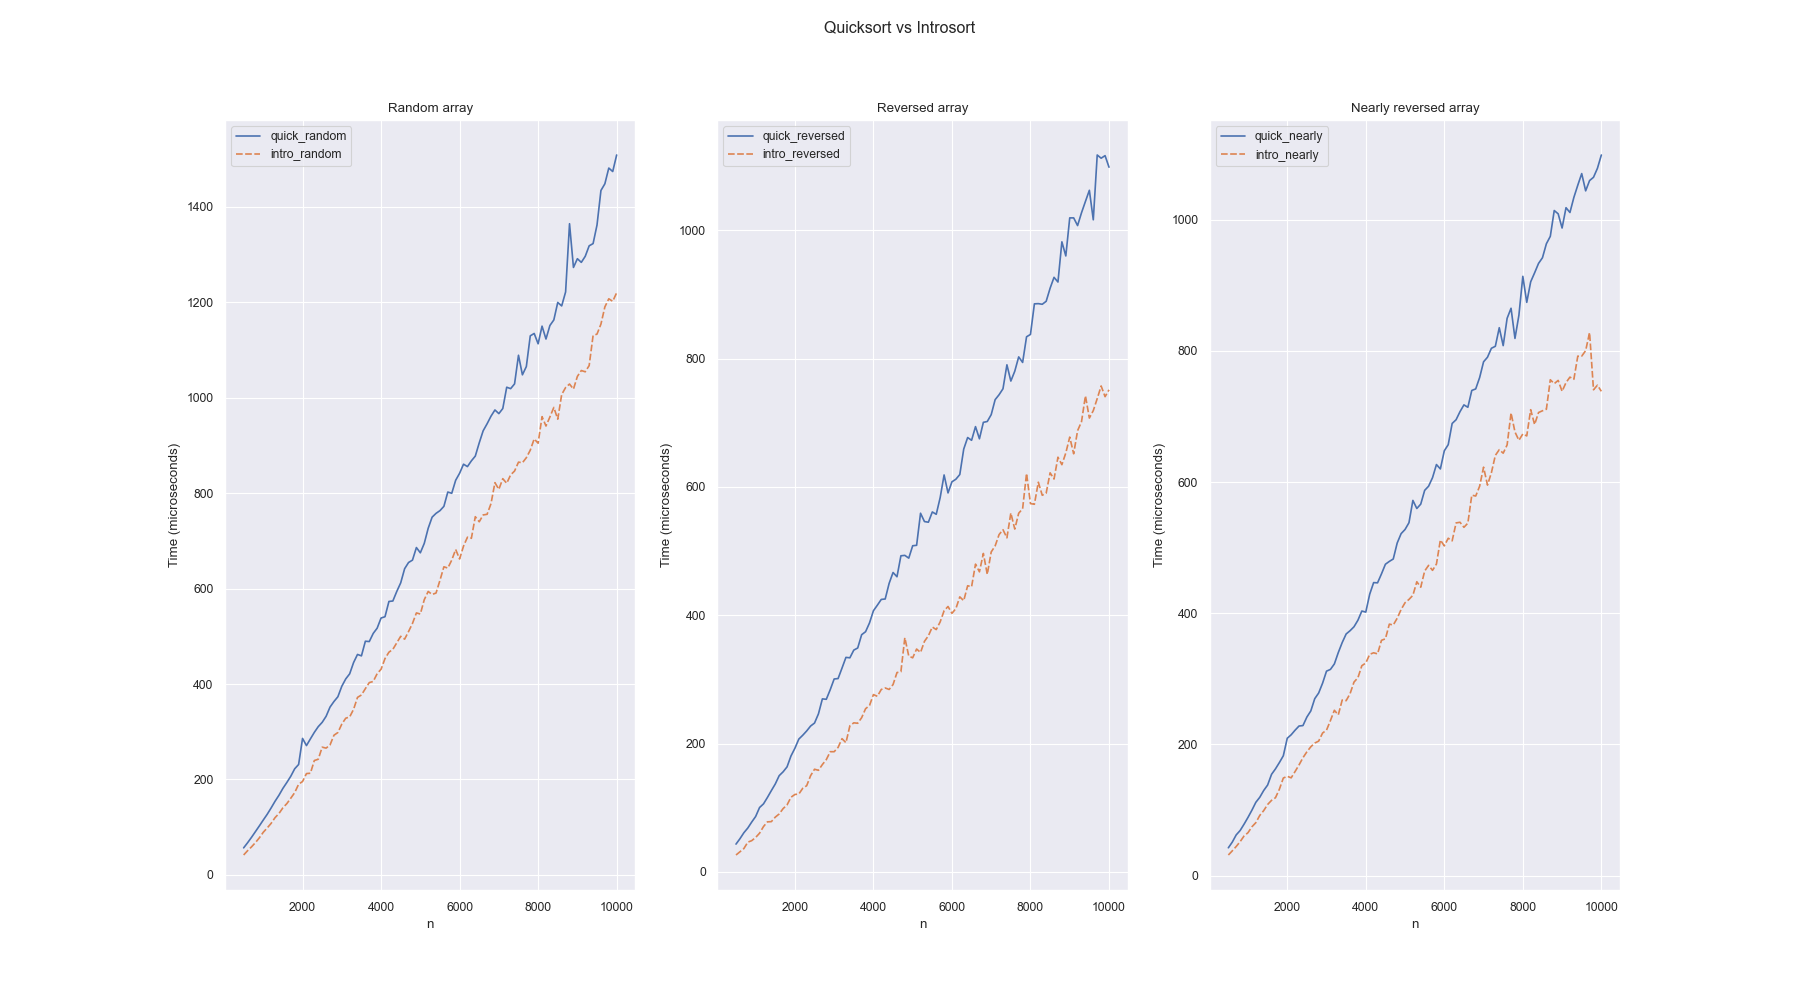
\includegraphics[width=0.85\textwidth]{../static/array_types.png}
	\caption{\texttt{IntroSort} \emph{vs.} \texttt{QuickSort}}
	\label{fig:types}
\end{figure}
\FloatBarrier

Результаты \emph{поражающие}! В каждом из случаев \texttt{IntroSort} показывает результат лучше другого алгоритма. Все это благодаря тому, что гибридная сортировка сочетает в себе достоинства трех различных алгоритмов.

\section*{Выводы}

Основные выводы по графикам были сделаны выше, тут же только отметим, что  при выборе между этими двумя сортировками стоит использовать вариант \texttt{IntroSort}.

\end{document}

